\documentclass{article}
\usepackage[utf8]{inputenc}
\usepackage[backend=biber]{biblatex}
\usepackage{amssymb}
\usepackage{amsmath}
\usepackage{dsfont}
\addbibresource{bib.bib}
\setlength{\parindent}{0em}
\bibliography{bib}
\setlength{\parskip}{6pt}
\usepackage[margin=1.0in]{geometry}
\usepackage{graphicx}
\usepackage{caption}
\usepackage{subcaption}
\usepackage{wrapfig}
\usepackage{url}

\title{Intro to deep learning with PyTorch}
\author{Miguel A. Saavedra-Ruiz}
\date{May 2020}
\linespread{1.0}

\nocite{*}


\begin{document}

\maketitle

\section*{Convolutional Neural Networks}

Convolutional Neural Networks (CNNs) are a variation of neural networks with the ability to efficiently operate over images. CNNs can look at images as a whole and learn to identify spatial patterns such as prominent colors and shapes, or whether a texture is fuzzy or smooth and so on. The shapes and colors that define any image and any object in an image are often called \textbf{features} Fig. \ref{fig:f1}.

An example of a feature would be what do we look at to distinguish a cat and a dog. These characteristics might be the shape of the eyes, the size, and how they move are just a couple of examples of visual features. 

\begin{figure}[ht]
    \centering
    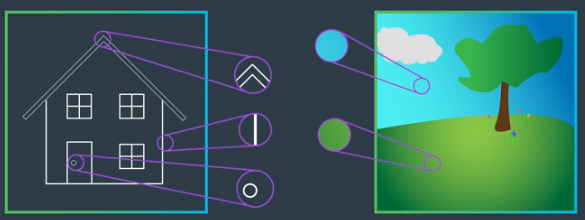
\includegraphics[width=0.45\textwidth,height=0.45\textheight,keepaspectratio]{images/features.png}
    \captionsetup{justification=centering}
    \caption{Features in an image}
    \label{fig:f1}
\end{figure}

To understand neural networks, it is important to also understand how an image is represented in a computer. In the case of gray scale images, these are interpreted by a computer as an array. A grid of values for each grid cell is called a pixel, and each pixel has a numerical value. In the MNIST database, each image is 28 pixels height and wide. Therefore, these images are understood by a computer as a 28 by 28 array. In a typical gray scale image, white pixels are encoded as the value 255, and black pixels are encoded as zero. Gray pixels fall somewhere in between, with light-gray being closer to 255. This description can be easily undertood with Fig. \ref{fig:f2}

\begin{figure}[ht]
    \centering
    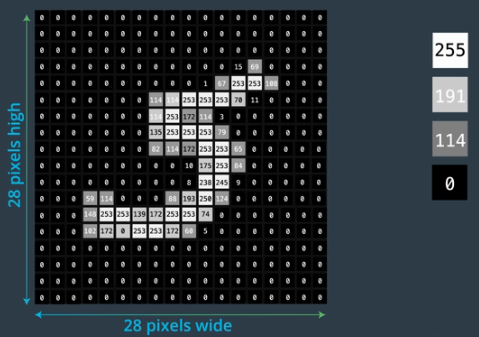
\includegraphics[width=0.4\textwidth,height=0.4\textheight,keepaspectratio]{images/image_representation.png}
    \captionsetup{justification=centering}
    \caption{Image representation as a matrix}
    \label{fig:f2}
\end{figure}

Nevertheless, the images in the MNIST dataset have actually gone through a quick pre-processing step. They've been re-scaled so that each image has pixel values in a range from zero to one Fig. \ref{fig:f3}. To go from a range of 0-255 to zero and one, it is necessary to divide every pixel value by 25 Eq. \eqref{eq:1}5. This step is called \textbf{normalization}.

\begin{figure}[ht]
    \centering
    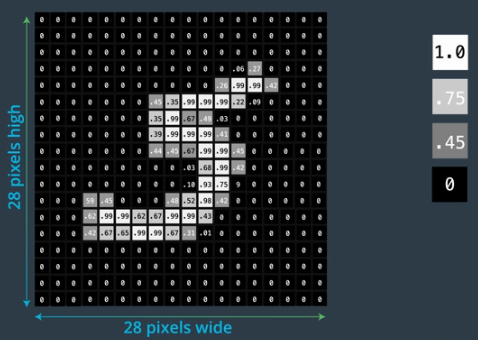
\includegraphics[width=0.4\textwidth,height=0.4\textheight,keepaspectratio]{images/image_norm.png}
    \captionsetup{justification=centering}
    \caption{Image representation as a normalized matrix}
    \label{fig:f3}
\end{figure}

\begin{equation}
NormX_{ij} = \frac{X_{ij}}{max(X)} \label{eq:1}
\end{equation}

Normalization is a useful tool to help the algorithm to train better. Thiss tep is quite useful due to neural networks rely on gradient calculations. These networks are trying to learn how important or how weighty a certain pixel should be in determining the class of an image. Normalizing the pixel values helps these gradient calculations stay consistent, and not get so large that they slow down or prevent a network from training.

Recall that to classify objects, the most common technique used for this was to use a MLP or fully connected neural network. However, these networks require 1-dimensional data. Hence, it is necessary to convert any array image into a vector. This process is called \textbf{flattening} and can be seen in Fig. \ref{fig:f4}. In this example, a four-by-four image which is a matrix with 16 pixel values. Instead of representing this as a four-by-four matrix, it is possible to construct a vector with 16 entries, where the first first entries of the vector correspond to the first row of the old array. The second four entries correspond to the second row and so on.

\begin{figure}[ht]
    \centering
    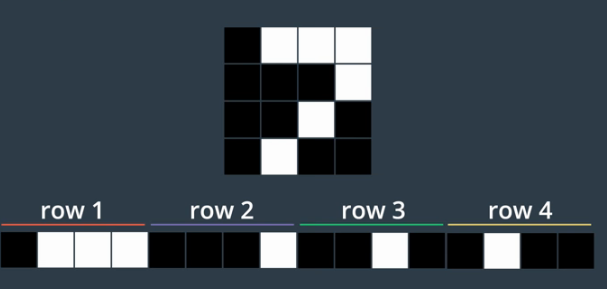
\includegraphics[width=0.4\textwidth,height=0.4\textheight,keepaspectratio]{images/flattening.png}
    \captionsetup{justification=centering}
    \caption{Flattening a simple matrix into a vector}
    \label{fig:f4}
\end{figure}

Once an image has been flattened, it is easy to pass the data to a MLP and obtain the classification result of the image.

It is important to note that Pytorch does Data normalization by subtracting the mean (the average of all pixel values) from each pixel, and then dividing the result by the standard deviation of all the pixel values.

\[\frac{P_{ij} - \mu}{\sigma}\]

Where for \(\mu = 0.5\) and \(\sigma=0.5\) the minimum (pixel coordinate equals 0) and maximum (pixel coordinate equals 1) values of the normalization are.

\[\frac{1 - 0.5}{0.5} = 1\]
\[\frac{0 - 0.5}{0.5} = -1\]

Resulting in a normalization of \([-1,1]\) for all the pixel values in the image.

A feasible network architecture to train the neural network is the one presented in Fig. \ref{fig:f50}. A MLP with 784 input units (number of inputs after flattening a MNIST image), two hidden layers with 512 nodes each and 10 output layers with a softmax activation function (one output per character) to produce a probability distribution in the final layer of the network.

\begin{figure}[ht]
    \centering
    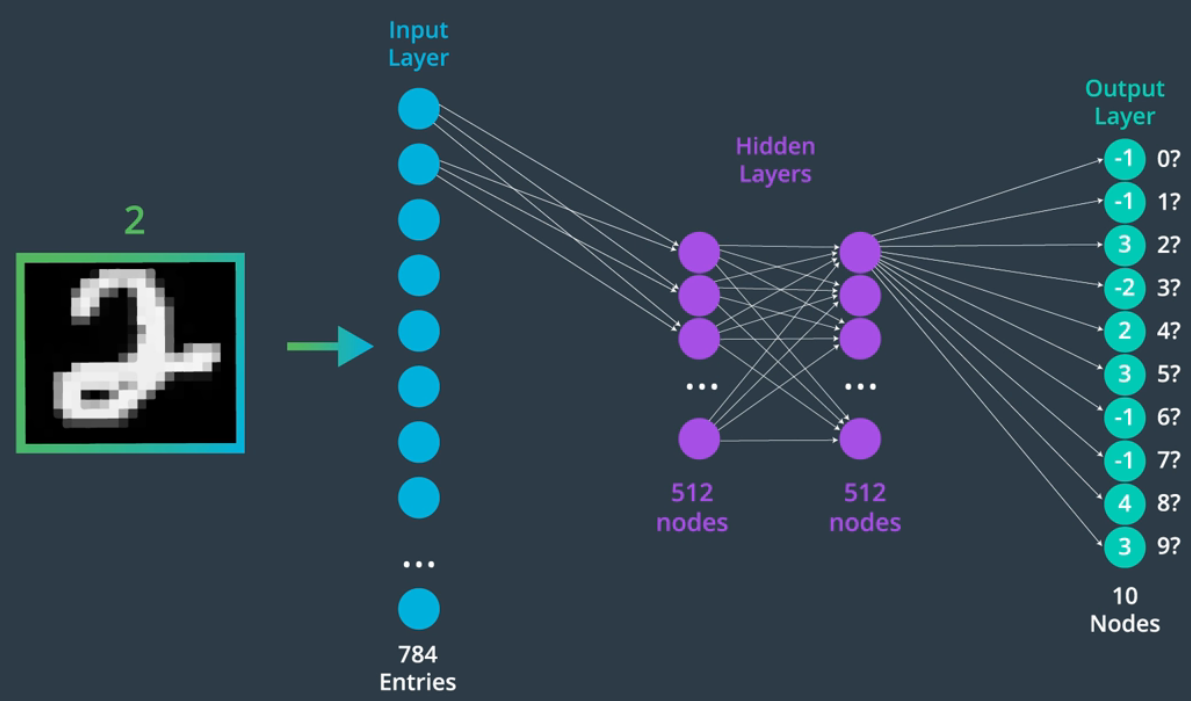
\includegraphics[width=0.55\textwidth,height=0.55\textheight,keepaspectratio]{images/mlp.png}
    \captionsetup{justification=centering}
    \caption{MLP to train a MNIST image}
    \label{fig:f5}
\end{figure}

Recall that neural networks learn from mistakes, hence, the next list of stems gives a gives of how to optimize the weights of a neural network.

\begin{enumerate}
  \item Loss: Measure any mistake between a predicted and true class
  \item Backpropagation: Quantify how bad a particular weight is in making a mistake
  \item Optimization: Gives a way to calculate a better weight value
\end{enumerate}

As this problem is categorized as a multi-classes problem, the \textbf{loss function} needed is called \textbf{categorical cross-entropy loss}. This loss function is defined as the negative log of the output layer (with softmax activation function).

Therefore, if the probability of a node is \(p(x_i) = 0.162\) the negative log is given in Eq. \eqref{eq:2}.

\begin{equation}
loss = -\log(0.162) = 1.82 \label{eq:2}
\end{equation}

If the probability is something like \(p(x_i) = 0.441\), then the loss would be \(loss = 0.819\)

It is possible to conclude that the categorical cross-entropy loss is \textbf{lower} when the prediction and label agree and \textbf{higher} when the prediction and label disagree (a probability close to one yields to a low loss value).

The optimizer is used to minimize the error of the loss function and change the weights towards the minimum error expression. In the Fig. \ref{fig:f6}, in the top right box it is possible to see a list of different optimizer and their performance minimizing the error. Each optimizer has its own benefits and the selection of one or other depends on the problem.

\begin{figure}[ht]
    \centering
    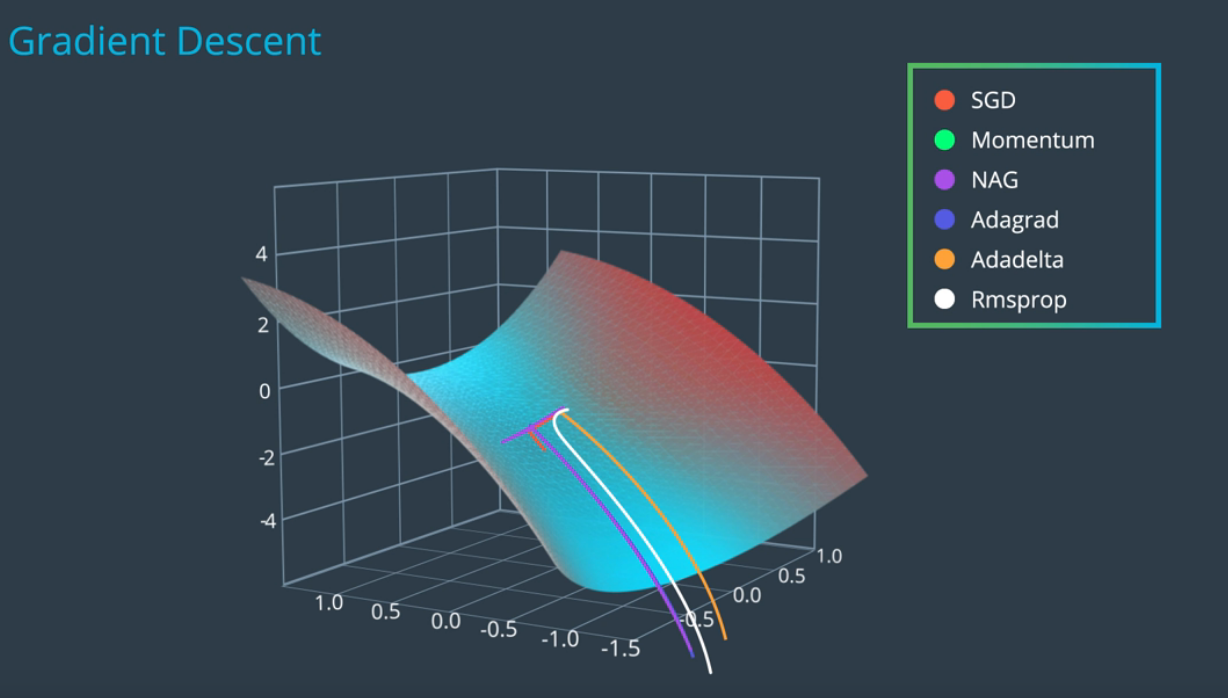
\includegraphics[width=0.4\textwidth,height=0.4\textheight,keepaspectratio]{images/optimizer.png}
    \captionsetup{justification=centering}
    \caption{Optimizer used to train a neural network}
    \label{fig:f6}
\end{figure}

A complete solution to the problem described before can be seen in \textit{mnist\_mlp\_exercise.ipynb}.

To decide whether the model is doing well or bad during training, a new set needs to be introduced. \textbf{The validation set} is defined as a sub-sample of the training set, usually the 20\% of the training set. During training, the training set is used to change the weights and the validation set checks the performance of the model to avoid over-fitting. Finally, once a model has been chosen, a test set is used (this set has never been seen by the network before) to check the accuracy of the trained model. The pipeline described before can be seen in Fig. \ref{fig:f7}.

\begin{figure}[ht]
    \centering
    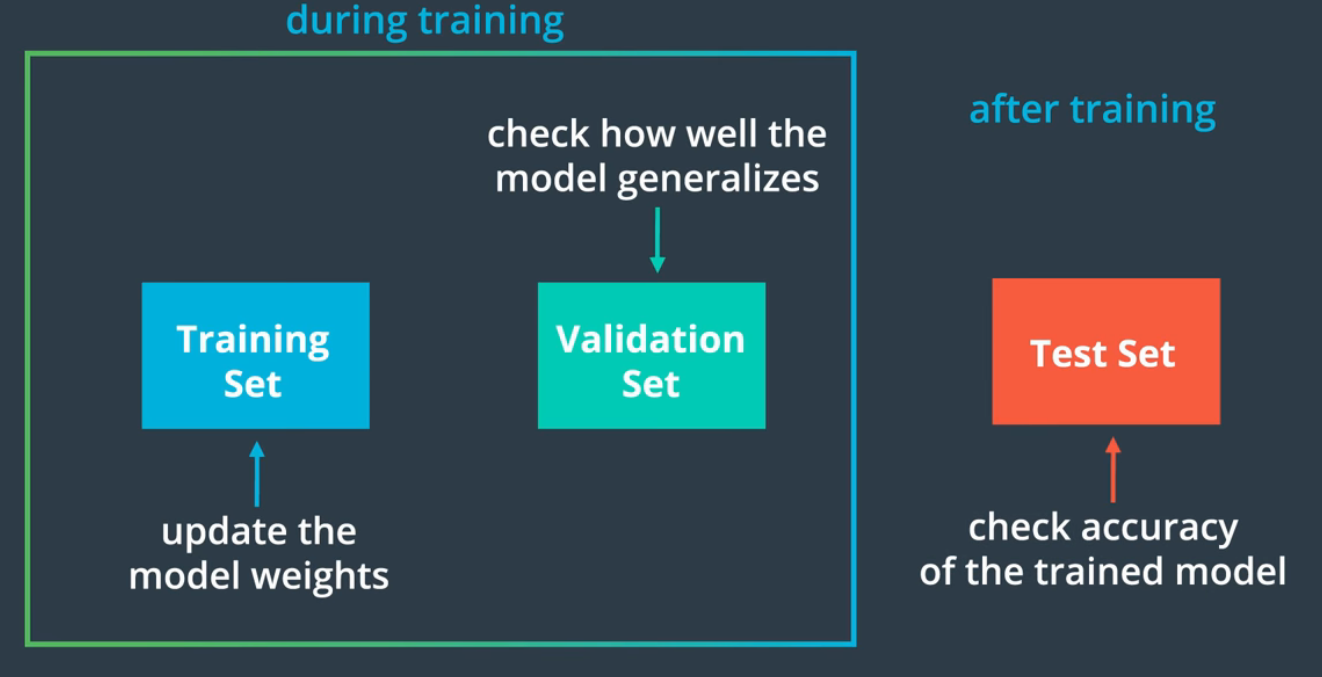
\includegraphics[width=0.55\textwidth,height=0.55\textheight,keepaspectratio]{images/sets.png}
    \captionsetup{justification=centering}
    \caption{Sets the evaluate and train a model}
    \label{fig:f7}
\end{figure}

Overall, the steps to train a neural network are:

\begin{itemize}
  \item Visualize data
  \item Pre-process normalize transform
  \item Define a model
  \item Train the model define loss \& optimization function
  \item Save the best model
  \item Test the model
\end{itemize}

Despite that flattening images and using multi-layer perceptrons might sound like a good solution to deal with images, these techniques have a set of drawbacks which affects its implementation in real world images. For example, the MLP only uses fully-connected layers, which for the case of the MNIST dataset is almost half a million parameters. Furthermore, this sort of architecture only support data in the form on vectors whereas the image is a matrix with spatial information which can be relevant around its close neighborhood. 

To sort this problems a new architecture is employed and this is \textbf{called convolutional neural networks (CNNs)}. This networks instead of use fully connected layers use sparsely connected layers where the connection between layers are informed by the 2-D structure of the image matrix. Moreover, this network architecture accepts matrices as inputs. 

To understand the concept of sparsely connected and its benefits, consider breaking the image into four regions Fig. \ref{fig:f8}. The image is painted in four sections: red, green, yellow, and blue. Then, each hidden node could be connected to only the pixels in one of these four regions.Here, each headed node sees only a quarter of the original image. With this regional breakdown and the assignment of small local groups of pixels to different hidden nodes, every hidden node finds patterns in only one of the four regions in the image. Then, each hidden node still reports to the output layer where the output layer combines the findings for the discovered patterns learned separately in each region

\begin{figure}[ht]
    \centering
    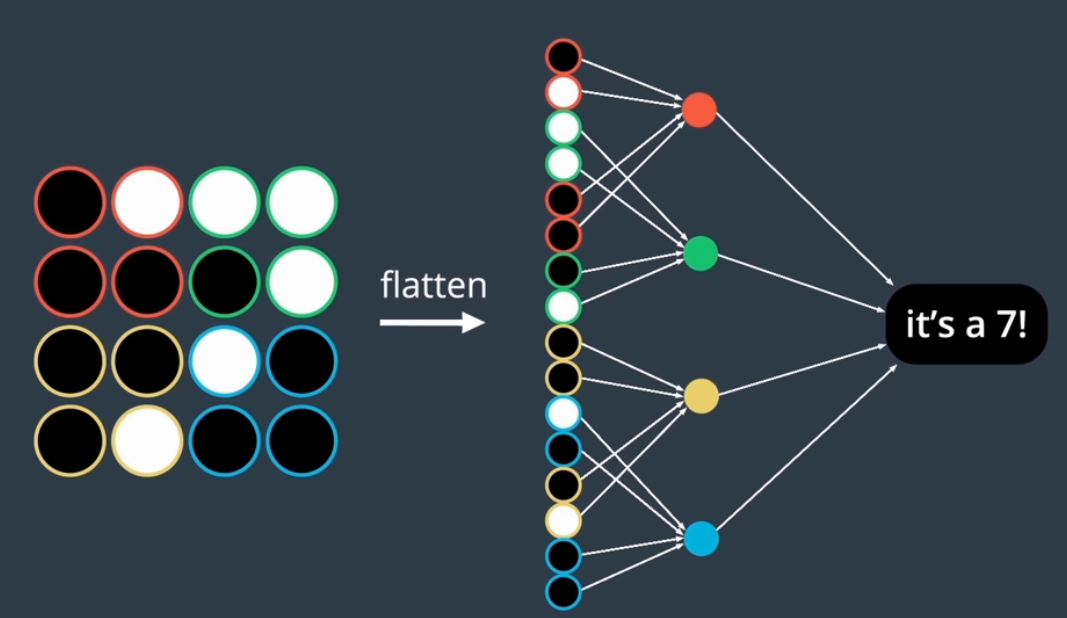
\includegraphics[width=0.55\textwidth,height=0.55\textheight,keepaspectratio]{images/sparsely.png}
    \captionsetup{justification=centering}
    \caption{Sets the evaluate and train a model}
    \label{fig:f8}
\end{figure}

This locally connected layer uses far fewer parameters than a densely connected layer. It's less prone to overfitting and truly understands how to tease out the patterns contained in image data. 

Rearranging the vector as a matrix it is possible to see the relationships between the nodes in each layer. It is possible to expand the number of patterns that the network is able to detect while still making use of the 2-D structure to selectively and conservatively add weights to the model by introducing more hidden nodes, where each is still confined to analyzing a single small region within the image. The red nodes in the hidden layer are still only connected to the red nodes in the input layer, with the same color coding for all other colors Fig. \ref{fig:f9}. 

\begin{figure}[ht]
    \centering
    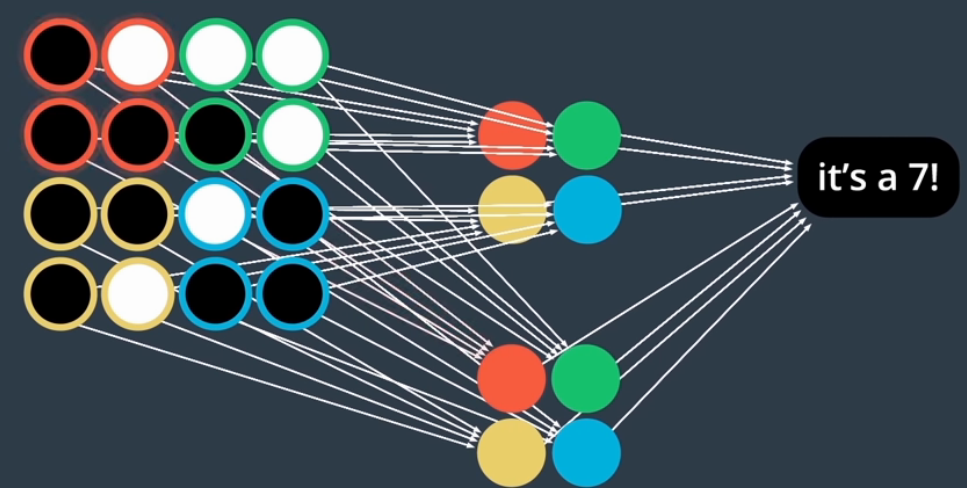
\includegraphics[width=0.55\textwidth,height=0.55\textheight,keepaspectratio]{images/matrix_input.png}
    \captionsetup{justification=centering}
    \caption{Arranging the matrix as an input for a CNNs}
    \label{fig:f9}
\end{figure}

Recall that by expanding the number of nodes in the hidden layer it is possible to discover more complex patterns in the data. In this case, two collections of hidden nodes is being used where each collection contains nodes responsible for examining a different region of the image as shown by Fig. \ref{fig:f10}. It will prove useful to have each of the hidden nodes within a collection share a common group of weights. The idea being that different regions within the image can share the same kind of information. In other words, every pattern that's relevant towards understanding the image could appear anywhere within the image.

\begin{figure}[ht]
    \centering
    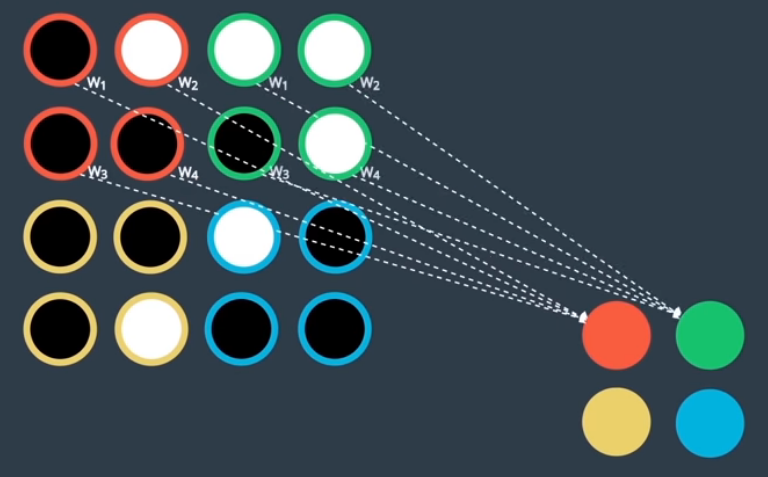
\includegraphics[width=0.55\textwidth,height=0.55\textheight,keepaspectratio]{images/shared_weights.png}
    \captionsetup{justification=centering}
    \caption{Sharing weights in a CNNs}
    \label{fig:f10}
\end{figure}

A convolutional neural network is a special kind of neural network which can remember spatial information. The common neural networks only look at individual inputs, whereas convolutional neural networks, can look at an image as a whole, or in patches and analyze groups of pixels at a time.

The key to preserving the \textbf{spatial information} in CNNs is called the convolutional layer. A \textbf{convolutional layer} applies a series of different image filters also known as \textbf{convolutional kernels} to an input image. The resulting filtered images have different appearances. The filters may have extracted features like the edges of objects in that image, or the colors that distinguish the different classes of images.

Spatial patterns in an image can be for example color or shape. The changes in shape can be described as the change of intensity in a group of pixels. These changes can be used to detect objects in an image. It is possible to identify these changes with convolutional kernels with a specific form and values.

To measure how the pixels change in an image, the frecuency can be used to identify the rate of change. A high frequency image Fig. \ref{fig:f11} is one where the intensity changes a lot  and the level of brightness changes quickly from one pixel to the next (pink square). A low frequency image may be one that is relatively uniform in brightness or changes very slowly (blue square). 

\begin{figure}[ht]
    \centering
    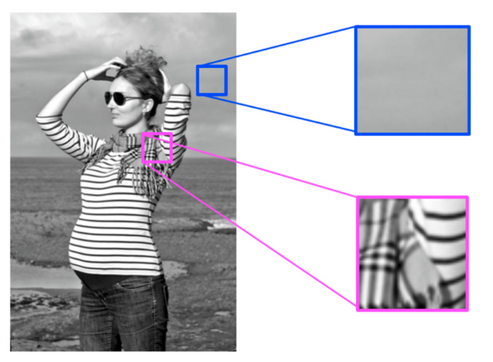
\includegraphics[width=0.55\textwidth,height=0.55\textheight,keepaspectratio]{images/frec.png}
    \captionsetup{justification=centering}
    \caption{High and low frecuency image patterns}
    \label{fig:f11}
\end{figure}

High-frequency components in an image also correspond to the edges of objects and can be used to classify them.

In an image, \textbf{filters} are used to filter out unwanted information or amplify features of interest as corners. An example of a filter is a high-pass filter which is used to sharpen an image and enhance high-frecuency parts of an image. In the Fig. \ref{fig:f12} the high-pass filter has enhanced the areas of the image where rapid changes have been presented (emphasizing edges). It is important to mention that this simple filters have to be used on one-channel images.


\begin{figure}[ht]
    \centering
    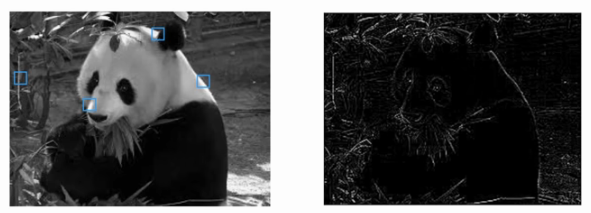
\includegraphics[width=0.55\textwidth,height=0.55\textheight,keepaspectratio]{images/high_pass.png}
    \captionsetup{justification=centering}
    \caption{Image after a High-pass filter}
    \label{fig:f12}
\end{figure}

A filter or convolutional filter is just a matrix of numbers that modifies the image. A high-ass filter is the one shown in Fig. \ref{fig:f13}. For edge detection, all the values inside the filter must add to zero.

\begin{figure}[ht]
    \centering
    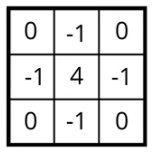
\includegraphics[width=0.2\textwidth,height=0.2\textheight,keepaspectratio]{images/filter.png}
    \captionsetup{justification=centering}
    \caption{High-pass filter}
    \label{fig:f13}
\end{figure}

To apply a filter to an image an operation called convolution needs to be applied to the image. In this operation, the kernel sweeps the whole image, multiplying value by value the pixel and kernel. Finally, all the values are added and the result is places in a new image which will counting the result of the convolution. The image Fig. \ref{fig:f14} shows this convolution process in a simple set of pixels in an image. Is is important to mention that the convolution is denoted by the symbol \(\*\).

\[K * I(x,y) = \text{resulting image}\]

\begin{figure}[ht]
    \centering
    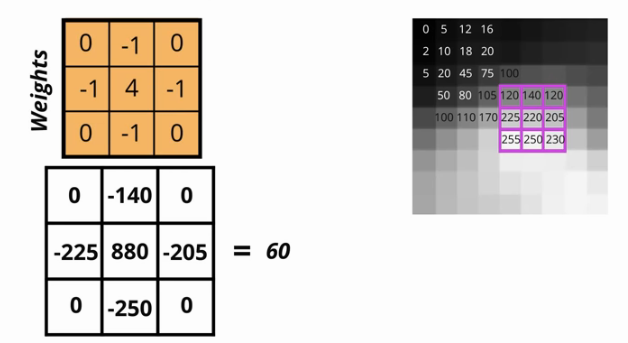
\includegraphics[width=0.55\textwidth,height=0.55\textheight,keepaspectratio]{images/convolution.png}
    \captionsetup{justification=centering}
    \caption{The convolution process}
    \label{fig:f14}
\end{figure}

When applying this process to the corners of an image leads to unknown pixel values, techniques as extend, padding or crop are applied in the input image to generate an image of the same size of the input one. 

Getting more into detail, CNNs are a kind of deep learning model that can learn to do things like image classification and object recognition. They keep track of spatial information and learn to extract features like the edges of objects in something called a convolutional layer. The Fig. \ref{fig:f15} shows a simple CNN structure, made of multiple layers.

\begin{figure}[ht]
    \centering
    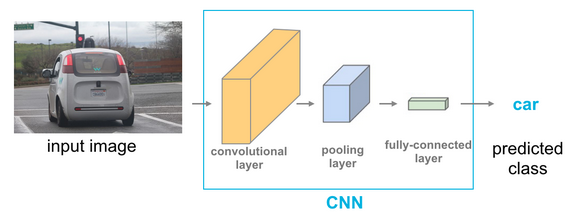
\includegraphics[width=0.65\textwidth,height=0.65\textheight,keepaspectratio]{images/layers_cnn.png}
    \captionsetup{justification=centering}
    \caption{Layers in a CNN}
    \label{fig:f15}
\end{figure}

The convolutional layer is produced by applying a series of many different image filters, also known as convolutional kernels, to an input image Fig. \ref{fig:f16}. In this case, four kernels mean four differently filtered output images.

\begin{figure}[ht]
    \centering
    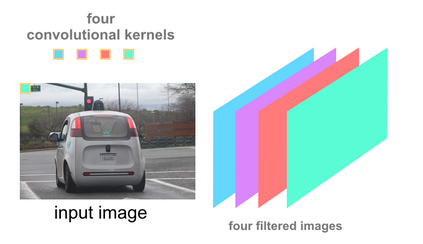
\includegraphics[width=0.55\textwidth,height=0.55\textheight,keepaspectratio]{images/conv_layer.png}
    \captionsetup{justification=centering}
    \caption{Convolutional layer}
    \label{fig:f16}
\end{figure}

When these outputs are stacked it is possible to form a complete convolutional layer with a depth of four Fig. \ref{fig:f17}

\begin{figure}[ht]
    \centering
    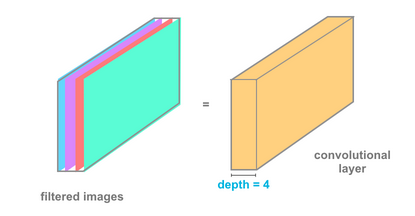
\includegraphics[width=0.45\textwidth,height=0.45\textheight,keepaspectratio]{images/depth.png}
    \captionsetup{justification=centering}
    \caption{Depth in a convolutional layer}
    \label{fig:f17}
\end{figure}

The main difference between a filter and a convolutional kernel is that neural networks will actually learn the best filter weights as they train on a set of image data. 

To see an example of a convolutional network in a grayscale image in pytorch, see the notebook \textit{conv\_visualization.ipynb}.

If the image has three channels (RGB) the filters need to be stacked in such way that there is a filter for each channel. This means that if the image has a depth of 3, the set of filters needed for this task will also have a depth of three. The result of this stacked filters will be the sum of the convolution of all the channels. Therefore for an input image with \(depth = 3\) and a set of filters \((20x4x4)\) where 20 is the amount of stacked filters and 4x4 is the size of the filter, the result will be a set of 20 images. A convolutional stacked filter can be seen in Fig. \ref{fig:f18}.

\begin{figure}[ht]
    \centering
    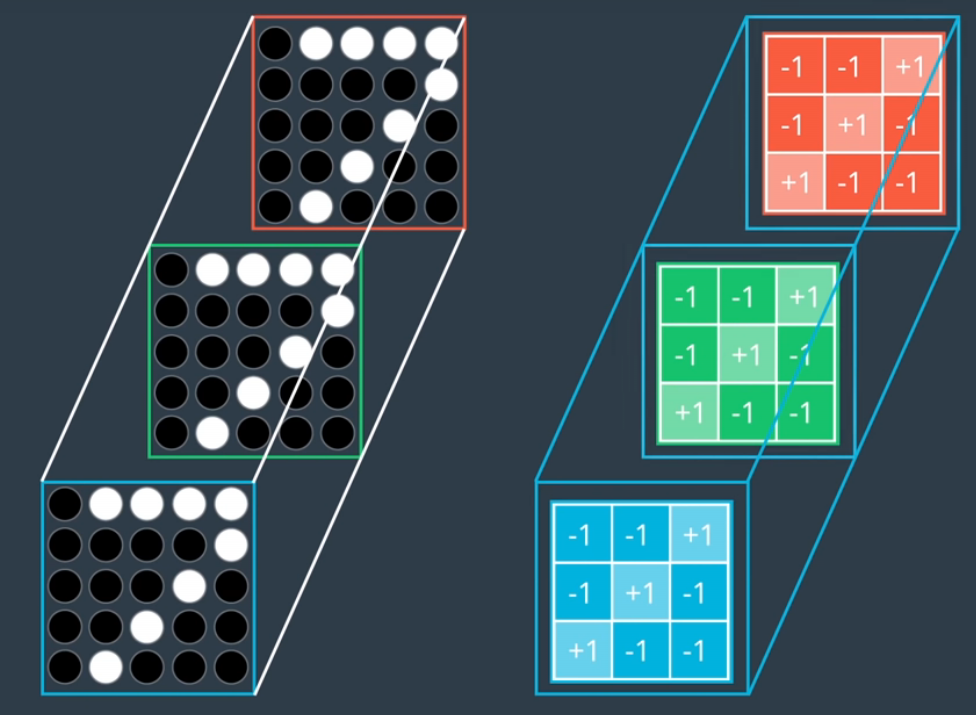
\includegraphics[width=0.45\textwidth,height=0.45\textheight,keepaspectratio]{images/conv_2d.png}
    \captionsetup{justification=centering}
    \caption{Convolution of RGB image}
    \label{fig:f18}
\end{figure}

In the Fig. \ref{fig:f19} is a brief explanation of how the filters operates through a 3-channels image to generate a single-channel output as the sum of the convolution of the three channels.

\begin{figure}[ht]
    \centering
    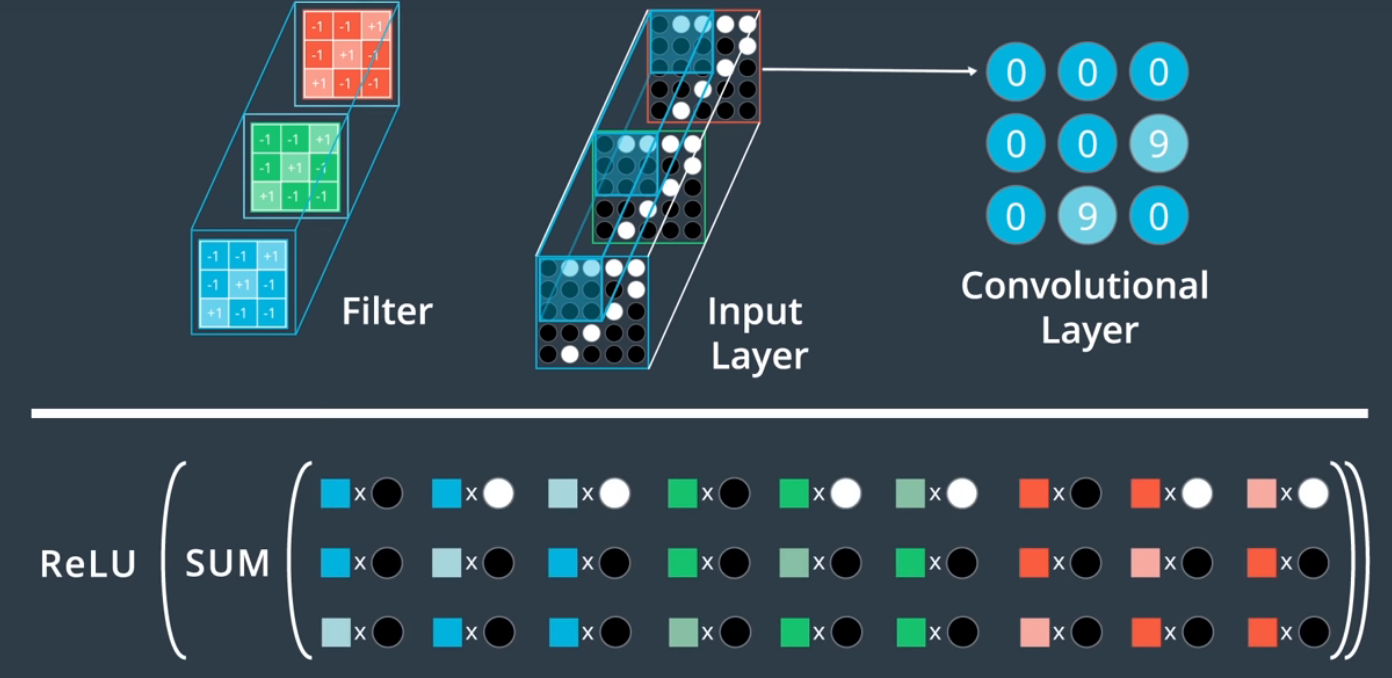
\includegraphics[width=0.75\textwidth,height=0.75\textheight,keepaspectratio]{images/conv_operation.png}
    \captionsetup{justification=centering}
    \caption{Result of a convolution with depth 3 is a image of one single channel}
    \label{fig:f19}
\end{figure}

It is important to mention that the multiple 2D outputs of a convolutional layer can be stacked together to generate inputs to more convolutional layers and discover more patterns among the patterns and improve the detection of features in the image. As the fully connected layers, convolutional layers have weights and bias (kernels) which are initially randomly generated and can be trained to achieve a specific task at hand. Overall, training a CNNs determine what kind of patterns it needs to detect based on the loss function, therefore, the filters will be learned based on the given data in the training process.

Besides the filter size and amount of filters, it is possible to tune additional parameters. One parameter is the \textbf{stride} and this is defined as the amount by which the filter slides over the image. For example, a stride of one means that the filter will slide only one pixel horizontally and vertically at each move. A stride of one will result in a feature map of almost the same size of the input image, whereas a stride of 2 will shrink the image in both width and height reducing the feature map size.

Another important parameter to use in CNNs is the \textbf{padding}. Zero padding can be added to an image with the objective to maintain the original image size in the output feature map. This process will allows a better extraction of features and avoid the loss of information in corners. To pad an image it is just necessary to add zeros in the surroundings of the image Fig. \ref{fig:f20}.

\begin{figure}[ht]
    \centering
    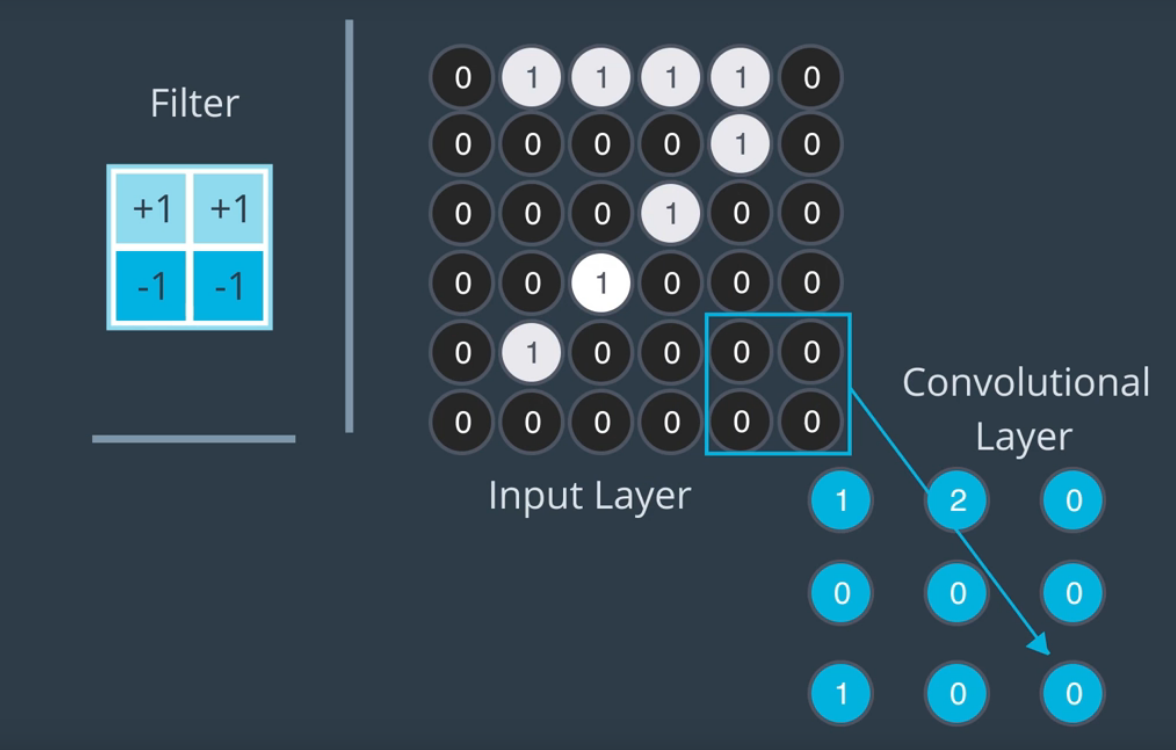
\includegraphics[width=0.5\textwidth,height=0.5\textheight,keepaspectratio]{images/padding.png}
    \captionsetup{justification=centering}
    \caption{Zero padding}
    \label{fig:f20}
\end{figure}

In Fig. \ref{fig:f15} is is possible to see that a CNN is composed of Convolutional layers, fully connected and pooling layers. \textbf{Pooling layers} are used as a method to reduce dimensionality and the amount of parameters after a convolution. There are basically two types of pooling layers. The first one is the max pooling layer and it works by just taking the maximum of the pixels contained in the window. Fig. \ref{fig:f21} shows an example of a max pooling layer which extracts the maximum value in each window. In this case, the stride of the max pooling is two. A max pooling layer reduce the size of the feature map to the half, reducing the amount of parameters in the neural network. An example of max pooling can be seen in the script \textit{maxpooling\_visualization.ipynb}.

\begin{figure}[ht]
    \centering
    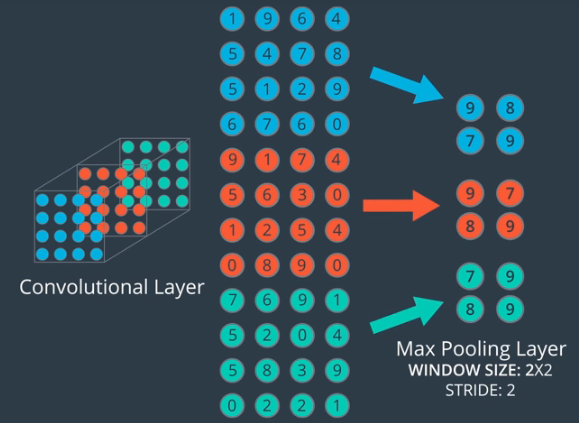
\includegraphics[width=0.5\textwidth,height=0.5\textheight,keepaspectratio]{images/max_pooling.png}
    \captionsetup{justification=centering}
    \caption{Max pooling in a feature map}
    \label{fig:f21}
\end{figure}

Overall, the general architecture of a convolutional neural network is a set con convolutional layers (with RELU activation function) and max pooling connected and finally flattened to feed a fully connected neural network Fig. \ref{fig:f22}

\begin{figure}[ht]
    \centering
    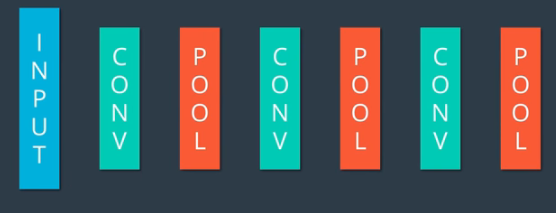
\includegraphics[width=0.4\textwidth,height=0.4\textheight,keepaspectratio]{images/architecture.png}
    \captionsetup{justification=centering}
    \caption{CNN common architecture}
    \label{fig:f22}
\end{figure}

It is quite important to recall that the max pooling layer is a good alternative to reduce parameter in a CNN. Nevertheless, it throws away some image information.


An alternative to classification methods that do not discard spatial information and instead learn to spatial relationships between parts is called \textbf{Capsule Networks}. This network architecture provide a way to detect parts of objects in an image and represent spatial relationships between those parts. This means that capsule networks are able to recognize the same object, like a face, in a variety of different poses and with the typical number of features (eyes, nose , mouth) even if they have not seen that pose in training data. 

Capsule networks are made of parent and child nodes that build up a complete picture of an object Fig. \ref{fig:f23}.

\begin{figure}[ht]
    \centering
    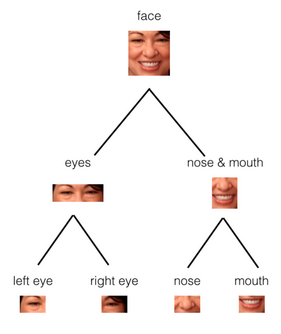
\includegraphics[width=0.3\textwidth,height=0.3\textheight,keepaspectratio]{images/faces.png}
    \captionsetup{justification=centering}
    \caption{Capsule Networks}
    \label{fig:f23}
\end{figure}

A very important pre-processing step in CNNs is to resize the images to the same image size. Typically, the images are resized as a square with the spatial dimension equal to a power of two \(2^x\). Fig. \ref{fig:f24} presents the general architecture of a CNN and this is as follows. It began with convolutional layers which detect regional patterns in an image using a series of image filters. Typically a ReLu activation function is applied to the output of these filters to standardize their output values. Then max pooling layers, which appear after convolutional layers to reduce the dimensionality of the input arrays. These new layers, along with fully-connected layers, are often the only layers used in this sort of networks.

\begin{figure}[ht]
    \centering
    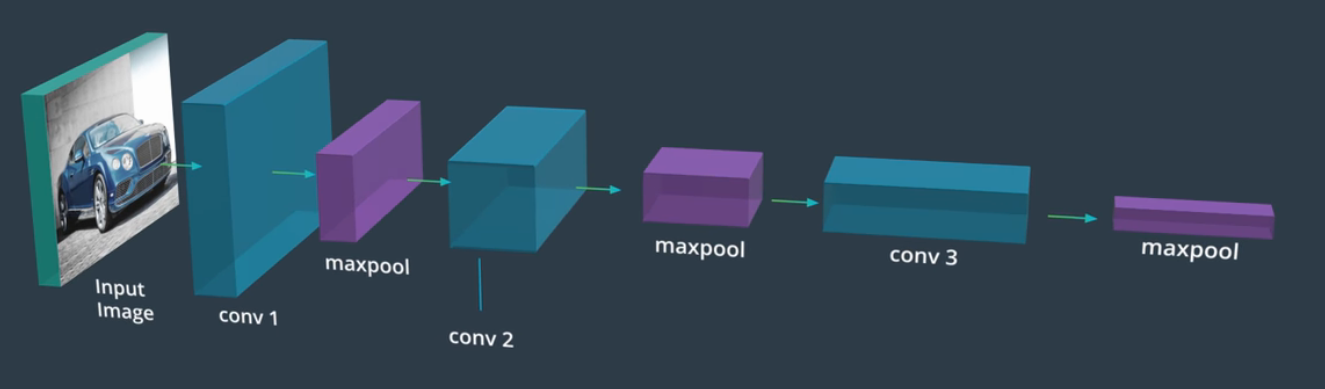
\includegraphics[width=0.6\textwidth,height=0.6\textheight,keepaspectratio]{images/full_cnn.png}
    \captionsetup{justification=centering}
    \caption{A complete CNN architecture}
    \label{fig:f24}
\end{figure}


It is possible to compute the spatial size of the output volume as a function of the input volume size (W), the receptive field size of the Conv Layer neurons (F), the stride with which they are applied (S), and the amount of zero padding used (P) on the border. The equation of the output is given by Eq. \eqref{eq:3}. For example for a 7x7 input and a 3x3 filter with stride 1 and pad 0 the output will be 5x5. With stride 2 the output would be 3x3.

\begin{equation}
\frac{W - F + 2P} {S} + 1
\label{eq:3}
\end{equation}

The number of parameters in a CNN is defined by Eq. \eqref{eq:4}, where \textbf{K} is the number of filters in the convolutional layer, \textbf{F} is the filter size, \textbf{\(D_{in}\)} corresponds to the depth of the previous layer and \textbf{K} is the bias term.

\begin{equation}
Param = K * F * F * D_{in}  + K
\label{eq:4}
\end{equation}

The idea behind the amount of layers in a CNNs is to extract the most revelant information of an image and finally, flatten it to construct a feature vector which can feed a fully connected layer. The general pipeline of a CNN with a fully connected layer is given in Fig. \ref{fig:f25}

\begin{figure}[ht]
    \centering
    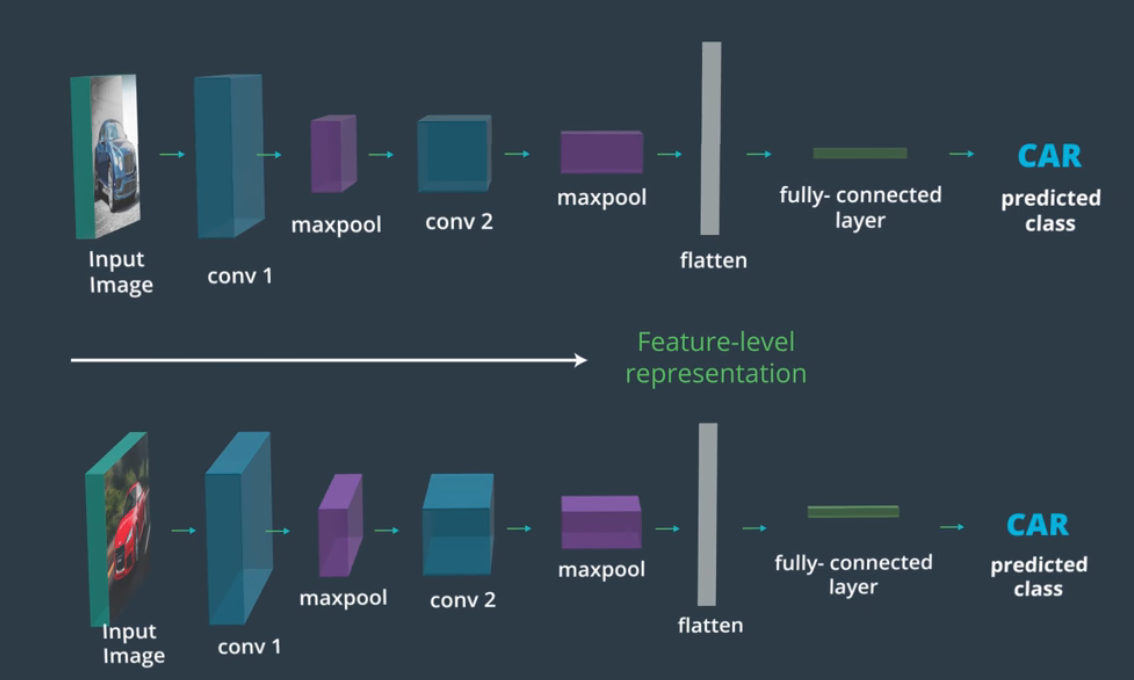
\includegraphics[width=0.75\textwidth,height=0.75\textheight,keepaspectratio]{images/fcn.png}
    \captionsetup{justification=centering}
    \caption{A complete CNN architecture with fully connected layers}
    \label{fig:f25}
\end{figure}

An implementation of a CNN can be seen in \textit{cifar10\_cnn.ipynb} where a fully convolutional neural network was used to classify the Cifar-10 dataset.

It is important that a CNN learns an invariant representation of the image which does not get affected by changes in scale, position, or angle in the interest object. Scale invariance is when the algorithm does not get affected by changes of size of the object in the image. Rotation invariance is immunity to change in the angle of the object in the image. Finally, translation invariance is when the algorithm is not affected by changes in the position of the object in the image frame.

To generate a CNN statically invariant and make it robust against those changes, it is necessary to apply a technique called \textbf{image augmentation}. This technique will allow the creation of artificial data with random rotation, translations and scale changes that will allow the algorithm to generalize better over different variations in an image. The Fig. \ref{fig:f26} shows an example of image augmentation in an image with an avocado, realizing changes in the position and orientation of the object. This technique is quite important because it prevents over fitting and improves generalization of the CNN.

\begin{figure}[ht]
    \centering
    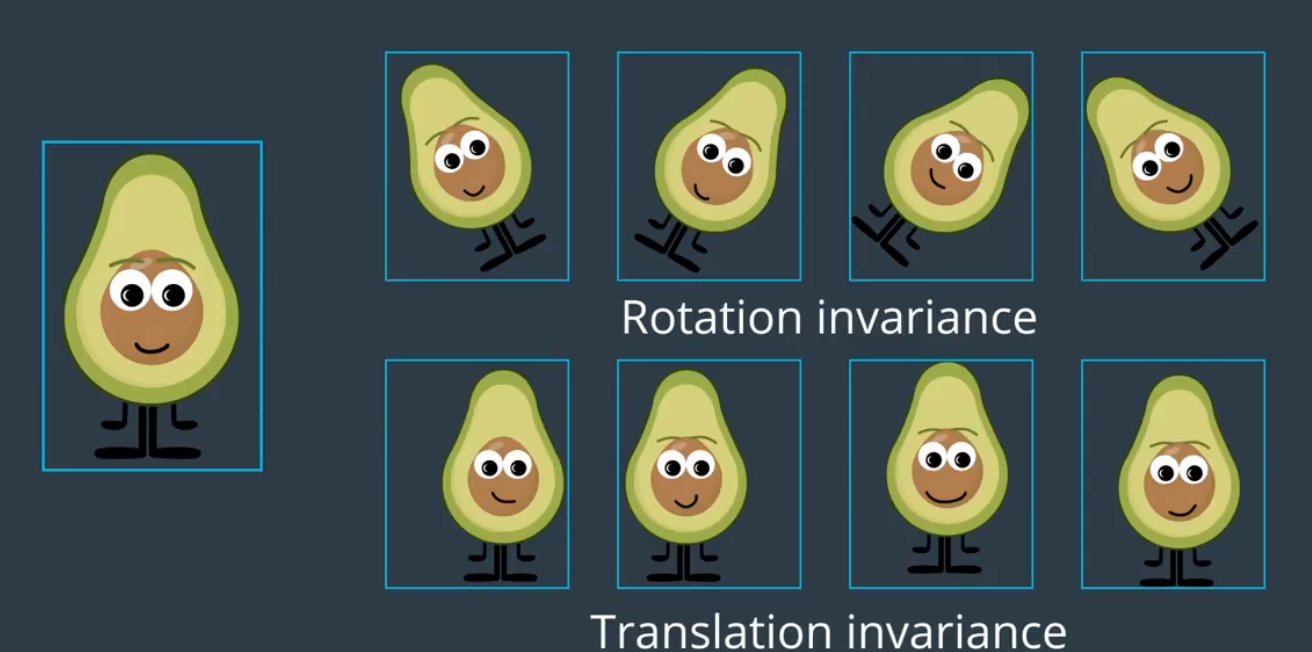
\includegraphics[width=0.6\textwidth,height=0.6\textheight,keepaspectratio]{images/augmentation.png}
    \captionsetup{justification=centering}
    \caption{Data augmentation}
    \label{fig:f26}
\end{figure}

The code \textit{cifar10\_cnn\_augmentation.ipynb} shows how to do image augmentation to improve generalization over a set of images.

\printbibliography

\end{document}
